%
% numerik.tex -- numerische Lösung von gewöhnlichen Differentialgleichungen
%
% (c) 2015 Prof Dr Andreas Mueller, Hochschule Rapperswil
%
\chapter{Numerische L"osung\label{chapter:numerik}}
\lhead{}
\rhead{Numerische L"osung}
\index{Numerische Loesung@Numerische L\"osung}
Im Kapitel~\ref{chapter:grundlagen} waren wir in der Lage, f"ur einige
einfache Differentialgleichungen eine L"osung in geschlossener Form
zu finden.
Zum Beispiel konnten wir lineare Differentialgleichungen mit Hilfe
der Exponentialfunktion l"osen.
Dieses Bild tr"ugt allerdings.
Die meisten Differentialgleichungen k"onnen nicht in geschlossener
Form gel"ost werden.
Wir k"onnen daher nicht erwarten, dass wir die L"osungen beliebiger
Differentialgleichungen einfach dadurch verstehen, dass wir
L"osungsfunktionen diskutieren.
Stattedessen bleiben uns nur die folgenden zwei M"oglichkeiten:
\begin{enumerate}
\item
Wir l"osen die Differentialgleichung mit Hilfe eines Computers,
und studieren den Verlauf der L"osungsfunktionen oder die Abh"angigkeit
von Parameter oder Anfangsbedingungen durch Vergleich verschiedener
numerisch gefundener L"osungen.
\item
Wir entwickeln Methoden, mit denen sich Aussagen "uber den Verlauf der
L"osungskurven studieren lassen, ohne dass man sie berechnet haben muss.
Nat"urlich kann man nicht erwarten, dass eine solche Methode genaue
Aussagen dar"uber erlaubt, wann eine L"osungskurve wo genau durchgehen
wird.
Es werden nur qualititative Aussagen m"oglich sein, zum Beispiel ob
Gleichgewichtsl"osunge stabil sind, ob es periodische L"osungen gibt
und ob L"osungskurven zu den periodischen L"osungen konvergieren.
\end{enumerate}
In diesem Kapitel entwickeln wir Methoden, Differentialgleichungen 
numerisch zu l"osen.

\section{Grundprinzip}
\begin{figure}
\centering
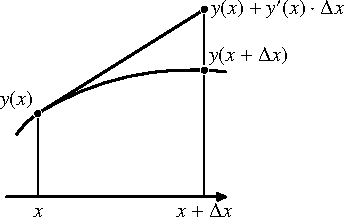
\includegraphics{chapters/images/numerik-2.pdf}
\caption{Lineare Approximation von $y(x+\Delta x)$ durch Information,
die am Punkt $x$ verf"ugbar ist.
\label{numerik:lineareapproximation}}
\end{figure}
Wir versuchen die Differentialgleichung
\begin{equation}
y'=-\alpha y,\qquad y(0)=y_0
\label{numerik:expdgl}
\end{equation}
numerisch zu l"osen. 
Dazu unterteilen wir die $x$-Achse in diskrete Abschnitte der L"ange $h$,
und bezeichnen die Teilpunkte mit $x_k=kh$.
Das Ziel ist jetzt, $y(x_k)$ n"aherungsweise zu berechnen.
Wir schreiben $y_k$ f"ur die N"aherungswerte von $y(x_k)$.
Die Ableitung liefert eine lineare Approximation f"ur $y(x)$,
n"amlich
\[
y(x+\Delta x)\simeq y(x) + y'(x)\cdot\Delta x
\]
(Abbildung~\ref{numerik:lineareapproximation}).
F"ur die Punkte $x_k$ bedeutet das
\[
y(x_{k+1})\simeq y(x_{k})+y'(x_k)\dot h.
\]
Die Differentialgleichung liefert Werte f"ur $y'(x_k)$ aus $x_k$ und $y(x_k)$,
damit k"onnen wir aus dieser Approximation ein allgemeines
N"aherungsverfahren f"ur die L"osung einer Differentialgleichung
konstruieren.

\begin{satz}[Euler-Verfahren]
Die Differentialgleichung
\begin{equation}
y'=f(x,y),\qquad y(0)=y_0
\label{numerik:eulerdgl}
\end{equation}
und die Schrittweite $h$ definieren eine Folge 
\[
y_{\mathstrut k}=y_{k-1} + h\cdot f(x_{k-1}, y_{k-1}),\quad k>0,
\]
mit $x_k=kh$,
die eine N"aherung f"ur die Funktionswerte $y(x_k)$ der L"osung $y(x)$
der Differentialgleichung~(\ref{numerik:eulerdgl}) ist.
\end{satz}

Dieses Verfahren ist nicht besonders gut, wie wir im Folgenden zeigen
wollen.
Die Diskussion soll uns aber zeigen, worauf bei der Weiterentwicklung
des Verfahrens geachtet werden muss.

Im vorliegenden Beispiel liefert die
Differentialgleichung~(\ref{numerik:expdgl})
den Wert $y'(x_k)=-\alpha y(x_k)$ f"ur die Ableitung,
woraus wir die Rekursionsformel
\[
y_{k+1}=y_k - \alpha y_k \dot h.
\]
gewinnen.
Die Rekursionsgleichung kann in diesem Fall exakt gel"ost werden,
und wir finden
\begin{equation}
y(x_{k+1}) = y(x_k)-\alpha y(x_k) h=(1-\alpha h) y(x_k)=\dots
=(1-\alpha h)^{k+1}y_0
\label{numerik:rekursion}
\end{equation}
f"ur die N"aherung $y_k$ der Funktionswerte $y(x_k)$.
%Angewendet auf eine beliebige Differentialgleichung, ist dieses
%einfache numerische Verfahren bekannt als das {\em Euler-Verfahren}.
%Es ist nicht besonders genau, aber soll in diesem Abschnitt dazu
%dienen, die Anforderungen an ein gutes numerisches Verfahren
%zu illustrieren.



Wir m"ochten $y(x)$ f"ur einen ganz bestimmten $x$-Wert berechnen.
Dazu unterteilen wir das Interval $[0,x]$ in $n$ Teilschritte der
Breite $x/n$, und wenden die Formel~(\ref{numerik:rekursion}) an:
\[
y(x)=y(x_n)=(1-\alpha h)^n y_0=\biggl(1+\frac{-\alpha x}{n}\biggr)^n y_0.
\]
F"ur eine grosse Zahl von Teilschritten erhalten wir so tats"achlich die
korrekte L"osung:
\[
\lim_{n\to\infty}y_0\biggl(1+\frac{-\alpha x}n\biggr)^n=y_0 e^{-\alpha x}.
\]
\begin{figure}
\centering
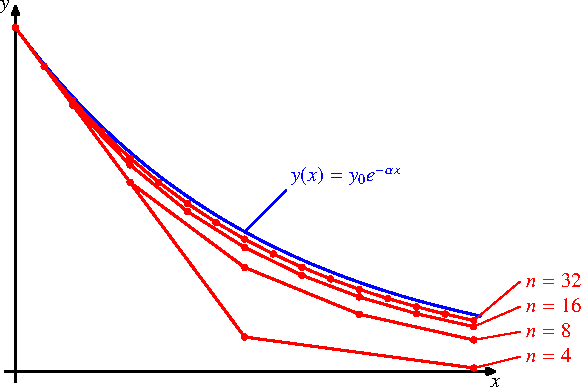
\includegraphics{chapters/images/numerik-1.pdf}
\caption{Approximationen der L"osung der Differentialgleichung $y'=-\alpha y$
mit verschiedener Anzahl Schritte (rot) n"ahern sich f"ur wachsendes
$n$ der exakten L"osung (blau).
\label{numerik:approximation}}
\end{figure}%
Abbildung~\ref{numerik:approximation} zeigt, wie die
durch~(\ref{numerik:rekursion}) gegebenen Approximationen mit zunehmendem
$n$ der exakten L"osung $y(x)=e^{-\alpha x}$ n"aher kommen.

Wir k"onnen auch den Fehler des numerischen Verfahrens berechnen.
Bei der Schrittweite $h$ ist der Fehler von $y_k$ die Differenz
\[
y(x_k)-y_k
=
y_0e^{-\alpha kh}-y_0(1-\alpha h)^k
=
y_0((e^{-\alpha h})^k - (1-\alpha h)^k)
=
y_0e^{-\alpha hk}\biggl(
1-\biggl(\frac{1-\alpha h}{e^{-\alpha h}}\biggr)^k
\biggr).
\]
Man beachte, dass der Z"ahler $1-\alpha h$ die Approximation
$y_1$ ist, als eine Approximation von $e^{-\alpha h}$, dem Nenner.
Schreiben wir
\[
q=\frac{1-\alpha h}{e^{-\alpha h}},
\]
f"ur den Quotienten zwischen der Approximation und dem korrekten Wert,
dann ist sicher immer $q<1$.
Den Fehler k"onnen wir jetzt schreiben
\[
y(x_k)-y_k = y_0e^{-\alpha hk}(1-q^k) = y(x_k)(1-q^k).
\]
Der relative Fehler des Verfahrens ist also
\[
\frac{y(x_k)-y_k}{y(x_k)}=(1-q^k).
\]
\begin{figure}
\centering
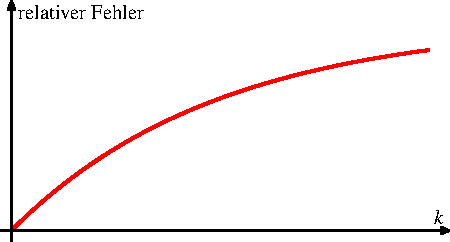
\includegraphics{chapters/images/numerik-3.pdf}
\caption{Relativer Fehler des Eulerverfahrens f"ur die Differentialgleichung
(\ref{numerik:expdgl}) in Abh"angigkeit von der Anzahl $k$ der Schritte.
\label{numerik:relfehler}}
\end{figure}%
Ganz unabh"angig von der Schrittweite $h$ wird der relative Fehler
des Verfahrens immer gegen 1 streben, der Fehler wird also von der
gleichen Gr"ossenordnung wie die berechneten Resultate.

Die Abbildung~\ref{numerik:relfehler} zeigt, dass zu Beginn des Verfahrens
der relative Fehler ungef"ahr linear mit der Anzahl der Schritt zunimmt.
Um eine angemessene Genauigkeit "uber einen gr"osseren Bereich
zu erreichen, muss das Euler-Verfahren also sehr viel kleinere Schritte
und eine entsprechend gr"ossere Anzahl von Schritten ausf"uhren,
die entsprechend viel Rechenzeit ben"otigen.

Ein praktisch n"utzliches Verfahren muss also anstreben, mit einer
sehr viel kleineren Anzahl von Schritten eine viel gr"ossere Genaugikeit
der Approximations zu erreichen.

\section{Fehler-Entwicklung numerischer L"osungen}
Wir betrachten wieder die Differentialgleichung~(\ref{numerik:eulerdgl})
und versuchen, den Fehler eines N"aherungsverfahrens zu bestimmen,
welches Schritte der Gr"osse $h$ durchf"uhrt, um den Wert $y(x)$
zu approximieren.

Das Euler-Verfahren verwendet Schritte der Form
\[
y_{k+1}=y_{k\mathstrut} + hf(x_{k\mathstrut},y_{k\mathstrut}}.
\]
In jedem einzelnen Schritt entsteht ein Fehler, dessen Gr"osse wir
aus der Taylor-Entwicklung
\[
y(x+\Delta x)=
y(x) + y'(x)\cdot \Delta x + R(x) \Delta x^2
\]
absch"atzen k"onnen.
Die Funktion $R(x)$ ist beschr"ankt und beschreibt den verbleibenden
Fehler.
Um $y(x)$ zu approximieren, m"ussen $n=x/h$ Schritte der Schrittweite
$h$ durchgef"uhrt werden, von denen jeder einen Fehler
von der Gr"ossenordnung $R(x)h^2$ hat.
Der Gesamtfehler ist daher von der Gr"ossenordnung
\[
y(x)-y_n=O\biggl(R(x)h^2\frac{x}h\biggr)=O(h),
\]
er ist also von erster Ordnung in $h$.
Um eine zus"atzliche Stelle Genauigkeit zu erhalten, muss man also zehnmal
so viele Schritte durchf"uhren, wodurch auch wieder Rundungsfehler
eingef"uhrt werden.

K"onnte man den Fehler des Einzelschrittes wesentlich verkleinern, w"urde
auch die Abh"angigkeit des Fehlers des Verfahrens vorteilhafter.
W"are der Fehler des Einzelschrittes $O(h^k)$ statt $O(h^2)$, dann
w"are der Gesamtfehler des Verfahrens nur noch $O(h^{k-1})$.
F"ur $k=3$ bedeutet dies, dass eine Halbierung der Schrittweite
zwar doppelt so viele Schritte braucht, aber auch, dass in jedem
Schritt nur ein Achtel des Fehlers auftritt.
Der Gesamtfehler ist also nur ein Viertel.
Mit zehnmal mehr Arbeit kann man also nicht nur eine Stelle an
Genauigkeit gewinnen, sondern gleich deren zwei.
Man spricht von einem quadratischen Verfahren oder einem Verfahren
zweiter Ordnung.
In der Praxis werden sogar Verfahren vierter und f"unfter Ordnung
verwendet, so dass eine zehnmal kleinere Schrittweite zu gleich
vier Stellen Genauigkeitsgewinn f"uhren.

\section{Einschritt-Verfahren}
\section{Mehrschritt-Verfahren}
\section{Finite Elemente}
